% Source : http://tex.stackexchange.com/questions/135801/depth-first-traversal-of-a-binary-tree/138799?noredirect=1#138799

\documentclass{article}
\usepackage{tikz}
\usetikzlibrary{calc, arrows}
\begin{document}
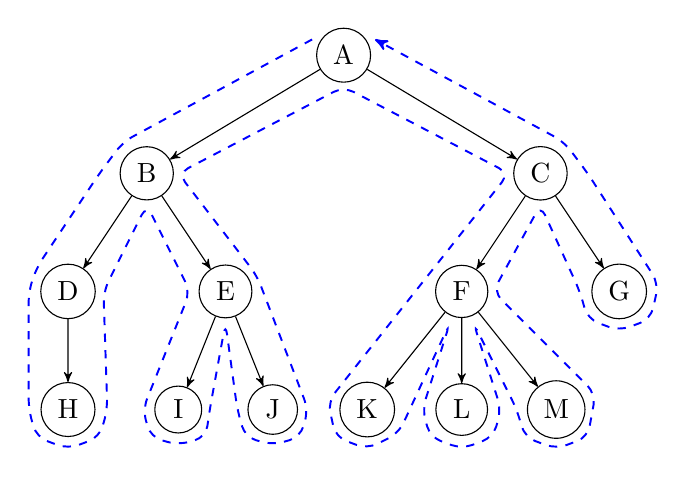
\begin{tikzpicture}[->,>=stealth',every node/.style={circle,draw},level 1/.style={sibling distance=50mm},level 2/.style={sibling distance=20mm},level 3/.style={sibling distance=12mm},
%scale=0.7, transform shape
]
\node (nA){A}
   child { node (nB) {B}
              child { node (nD) {D}
                         child { node (nH) {H} }
                       }
              child {  node (nE) {E}
                         child { node (nI) {I} }
                         child { node (nJ) {J} }
                       }
            }
   child { node (nC) {C}
              child { node (nF) {F}
                         child { node (nK) {K}  }
                         child { node (nL) {L} }
                         child { node (nM) {M} }
                       }
              child {  node (nG) {G} }
             };

  \draw[->,blue,rounded corners,dashed,line width=0.7pt]
    ($(nA)  +(-0.4,0.2)$) --
    ($(nB)  +(-0.3,0.4)$) --
    ($(nB)  +(-0.6,0.0)$) --
    ($(nD)  +(-0.4,0.3)$) --
    ($(nD)  +(-0.5,0.0)$) --
    ($(nH)  +(-0.5,0.0)$) --
    ($(nH)  +(-0.4,-0.35)$) --
    ($(nH)  +(0.0,-0.5)$) --
    ($(nH)  +(0.4,-0.35)$) --
    ($(nH)  +(0.5,0.0)$) --
%    ($(nD)  +(0.45,-0.2)$) --
    ($(nD)  +(0.45,0.0)$) --
    ($(nB)  +(0.0,-0.4)$) --
    ($(nE)  +(-0.45,0.0)$) --
    ($(nI)  +(-0.45,0.0)$) --
    ($(nI)  +(-0.35,-0.35)$) --
    ($(nI)  +(0.0,-0.45)$) --
    ($(nI)  +(0.35,-0.35)$) --
    ($(nI)  +(0.4,0.0)$) --
    ($(nE)  +(0.0,-0.4)$) --
    ($(nJ)  +(-0.45,0.0)$) --
    ($(nJ)  +(-0.35,-0.35)$) --
    ($(nJ)  +(0.0,-0.45)$) --
    ($(nJ)  +(0.35,-0.35)$) --
    ($(nJ)  +(0.45,0.0)$) --
    ($(nE)  +(0.4,0.2)$) --
    ($(nB)  +(0.4,0.0)$) --
    ($(nA)  +(0.0,-0.4)$) --
    ($(nC)  +(-0.4,0.0)$) --
%    ($(nF)  +(-0.6,0.0)$) --
    ($(nK)  +(-0.5,0.1)$) --
    ($(nK)  +(-0.4,-0.35)$) --
    ($(nK)  +(0.0,-0.5)$) --
    ($(nK)  +(0.4,-0.3)$) --
    ($(nF)  +(-0.15,-0.4)$) --
    ($(nL)  +(-0.5,0.0)$) --
    ($(nL)  +(-0.4,-0.35)$) --
    ($(nL)  +(0.0,-0.5)$) --
    ($(nL)  +(0.4,-0.35)$) --
    ($(nL)  +(0.5,0.0)$) --
    ($(nF)  +(0.15,-0.4)$) --
    ($(nM)  +(-0.5,0.0)$) --
    ($(nM)  +(-0.4,-0.35)$) --
    ($(nM)  +(0.0,-0.5)$) --
    ($(nM)  +(0.4,-0.35)$) --
    ($(nM)  +(0.5,0.2)$) --
    ($(nF)  +(0.4,0.0)$) --
    ($(nC)  +(0.0,-0.4)$) --
    ($(nG)  +(-0.5,0.0)$) --
    ($(nG)  +(-0.4,-0.35)$) --
    ($(nG)  +(0.0,-0.5)$) --
    ($(nG)  +(0.4,-0.35)$) --
    ($(nG)  +(0.5,0.1)$) --
    ($(nC)  +(0.6,0.0)$) --
    ($(nC)  +(0.3,0.4)$) --
    ($(nA)  +(0.4,0.2)$);
\end{tikzpicture}
\end{document}